\documentclass[10pt,conference]{IEEEtran}
\usepackage[utf8]{inputenc}
\usepackage[english]{babel}
\usepackage{enumitem}
\usepackage{biblatex}
\usepackage[utf8]{inputenc}
\usepackage{graphicx}
\usepackage{multirow}
\usepackage{caption} 

\usepackage{balance}
\usepackage[skins]{tcolorbox}

\addbibresource{msr-challenge.bib}
%\renewcommand\IEEEkeywordsname{Keywords}

\newlist{questions}{enumerate}{1}
\setlist[questions]{label*=\textbf{RQ\arabic*.}}

% correct bad hyphenation here
\hyphenation{op-tical net-works semi-conduc-tor}

\title{Can Continuous Integration Help Warn about One-line Bugs?}

\newcommand{\conclusion}[1]{\begin{center}\begin{tcolorbox}[skin=widget, left=0.5mm,right=0.5mm,top=0.5mm,bottom=0.5mm,boxrule=0.3mm,arc=0mm,coltitle=black,colframe=black!99!white,colback=white!88!gray,width=(\linewidth),before=\hfill,after=\hfill]#1\end{tcolorbox}\end{center}}

\newcommand{\linebreakand}{%
  \end{@IEEEauthorhalign}
  \hfill\mbox{}\par
  \mbox{}\hfill\begin{@IEEEauthorhalign}
}

\newcommand{\rqi}{RQ1:  How many bug-inducing commits does CI fail on?}
\newcommand{\rqii}{RQ2: Why aren't one-line bugs caught by CI?}

\begin{document}

% author names and affiliations
% use a multiple column layout for up to three different
% affiliations
\author{\IEEEauthorblockN{Jasmine Latendresse}
\IEEEauthorblockA{Concordia University\\
Department of Computer Science and\\
Software Engineering\\
Montreal, Canada\\
j\_latend@encs.concordia.ca}
\and
\IEEEauthorblockN{Rabe Abdalkareem}
\IEEEauthorblockA{Concordia University\\
Department of Computer Science and\\
Software Engineering\\
Montreal, Canada\\
INCLUDE EMAIL}
\and
\IEEEauthorblockN{Diego Elias Costa}
\IEEEauthorblockA{Concordia University\\
Department of Computer Science and\\
Software Engineering\\
Montreal, Canada\\
diego.costa@concordia.ca}
\linebreakand
\IEEEauthorblockN{Emad Shihab}
\IEEEauthorblockA{Concordia University\\
Department of Computer Science and\\
Software Engineering\\
Montreal, Canada\\
emad.shihab@concordia.ca}}

% make the title area
\maketitle

% As a general rule, do not put math, special symbols or citations
% in the abstract
\begin{abstract}
Continuous Integration (CI) is the practice of automatically compiling, building, and testing code changes from multiple contributors to be integrated into a single code base. Bug fixing is one of the core tasks in software development and becomes increasingly costly over time. Hence, the development community has adopted Continuous Integration (CI) as a way to push changes into production as quickly as possible by integrating often; allowing to detect and locate errors quickly. However, little is known about how effective Continuous Integration (CI) is at detecting simple, one-line bugs. Hence, in this paper, we analyze the coverage of Continuous Integration (CI), particularly, Travis CI---a popular CI service provider, of failed builds for simple, one-line bugs. We find that 15.72\% of the bug-inducing commits from open source projects are associated with a CI build and that only 10\% of the CI builds are flagged as failed after the bug-inducing commit is introduced to the code base. 
\end{abstract}

\begin{IEEEkeywords}
	One-line bug, Continuous Integration, Software Development
\end{IEEEkeywords}

\section{Introduction}
Continuous Integration (CI) is an increasingly popular practice adopted by the software industry to automate the compilation, building, testing, and deployment of software. With CI, incremental changes brought to the code base are more atomic which in theory makes bug detection simpler and quicker. Early bug detection and reporting significantly reduces overhead since it allows developers to fix faults and make possible critical decisions earlier in the project's lifecycle; having fewer unintended consequences.


\begin{questions}
    \item How many bug-inducing commits does CI fail on? \\ Our findings show that 10\% of the builds fail after the bug-inducing commit is introduced to the code base. 
\end{questions}
\begin{questions}[resume]
    \item Why aren't one-line bugs caught by the CI? \\ We find that 66.7\% of the failed builds preceding the fix commit introduction have no tests and that this proportion is reduced to 45.5\% after the fix commit introduction. 
\end{questions}

\section{Case Study Design}
In this section, we discuss each step of the approach that we use to analyze the mining challenge data set and address our research questions. An overview of our approach is shown in Figure~\ref{fig:process}.

\begin{figure*}[t]
\centering
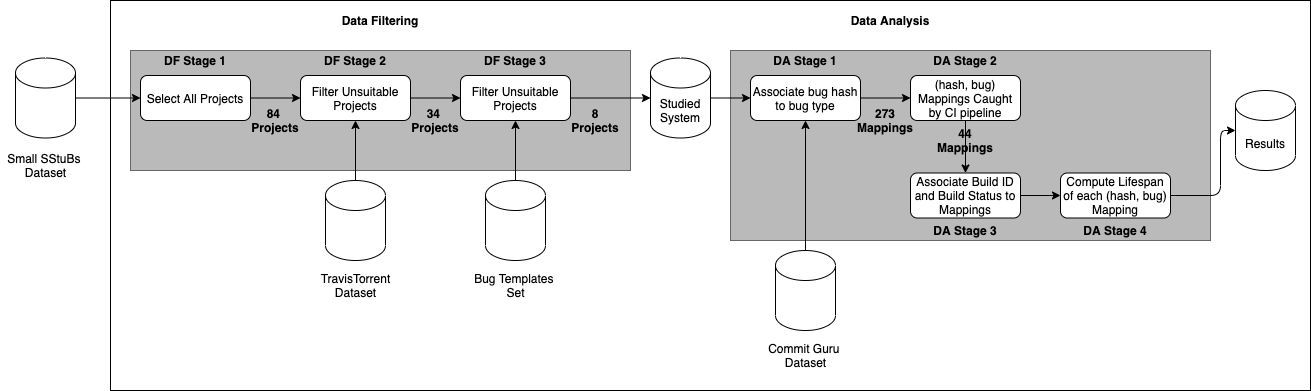
\includegraphics[width=\linewidth]{process.png}
\caption{An overview of our approach to study the MSR Challenge data set.}
\label{fig:process}
\end{figure*}

%How we selected the project for our analysis (how we filtered down to the 8 projects we have, what were the criteria, etc). Mention extraction of additional data from travis torrent and commit guru. Why we wanted travis torrent data (for CI data), why we needed commit guru data (to have additional data on the commit (bug) history.
\subsection{Data Filtering}
some text \\
\textbf{DF 1: some text \\}
\textbf{DF 2: some text \\}
\textbf{DF 3: some text \\}

\subsection{Data Analysis}
some text \\
\textbf{DA 1: some text \\}
\textbf{DA 2: some text \\}
\textbf{DA 3: some text \\}
\textbf{DA 4: some text \\}

\section{Case Study Results}
In this section, we present the results of our case study with respect to the three research questions. For each research question, we present the motivation for the question, the approach to answer the question, and results.

\subsection*{\rqi}

\noindent\textbf{Motivation:}

\noindent\textbf{Approach:}

\noindent\textbf{Result:}

\conclusion{Summary of the findings of this RQ}

\subsection*{\rqii}

\noindent\textbf{Motivation:}


\noindent\textbf{Approach:}


\noindent\textbf{Result:}

\conclusion{Summary of the findings of this RQ}

\begin{table*}[t]
\centering
\begin{tabular}{lll|lll}
\hline
\multicolumn{3}{l|}{}                                      & Failed tests & Passed tests & No tests \\ \hline
\multirow{3}{*}{tr\_build\_status} & Pass  & 82\% & 0\%          & 78,05\%      & 21,95\%  \\
                                            & Fail  & 10\% & 60\%         & 20\%         & 20\%     \\
                                            & Error & 36\% & 6\%          & 16,67\%      & 77,78\%  \\ \hline
\end{tabular}
\label{tab:bugintro}
\caption{Build status of Travis CI builds at bug-inducing commit introduction. \\ (Traceability--50 builds)}
\end{table*}

% Please add the following required packages to your document preamble:
% \usepackage{multirow}
\begin{table*}[t]
\centering
\begin{tabular}{lll|lll}
\hline
\multicolumn{3}{l|}{}                                & Failed tests & Passed tests & No tests \\ \hline
\multirow{3}{*}{tr\_build\_status} & Pass  & 89,47\% & 5,88\%       & 68,63\%      & 25,49\%  \\
                                   & Fail  & 5,26\%  & 33\%         & 0\%          & 66,67\%  \\
                                   & Error & 5,26\%  & 0\%          & 33,33\%      & 66,67\%  \\ \hline
\end{tabular}
\label{tab:beforefix}
\caption{Build Status of Travis CI builds before the fix commit is introduced. \\ (Traceability--57 builds)}
\end{table*}

\begin{table*}[t]
\centering
\begin{tabular}{lll|lll}
\hline
\multicolumn{3}{l|}{}                                & Failed tests & Passed tests & No tests \\ \hline
\multirow{3}{*}{tr\_build\_status} & Pass  & 83,33\% & 1,64\%       & 70,07\%      & 28,62\%  \\
                                   & Fail  & 12,02\% & 34,09\%      & 20,45\%      & 45,45\%  \\
                                   & Error & 4,64\%  & 0\%          & 23,53\%      & 76,47\%  \\ \hline
\end{tabular}
\label{tab:afterfix}
\caption{Build Status of Travis CI builds after the fix commit is introduced. \\ (Traceability--366 builds)}
\end{table*}

\begin{table*}[t]
\begin{tabular}{llll}
\hline
Bug Type                           & Average Lifespan (days) & Median Lifespan (days) & Number of instances associated with a CI build \\ \hline
CHANGE\_IDENTIFIER                 & 57.0                    & 10.0                   & 16                                             \\
DIFFERENT\_METHOD\_SAME\_ARGS      & 68.1                    & 6.7                    & 6                                              \\
CHANGE\_MODIFIER                   & 202.8                   & 6.8                    & 5                                              \\
CHANGE\_NUMERAL                    & 31.23                   & 6.1                    & 4                                              \\
CHANGE\_CALLER\_IN\_FUNCTION\_CALL & 5.6                     & 5.6                    & 3                                              \\
SWAP\_BOOLEAN\_LITERAL             & 89.4                    & 89.4                   & 2                                              \\
OVERLOAD\_METHOD\_MORE\_ARGS       & 110.2                   & 110.2                  & 1                                              \\
LESS\_SPECIFIC\_IF                 & 10.6                    & 10.6                   & 1                                              \\
OVERLOAD\_METHOD\_DELETED\_ARGS    & 68.6                    & 68.6                   & 1                                              \\
SWAP\_ARGUMENTS                    & 0.9                     & 0.9                    & 1                                              \\
CHANGE\_OPERAND                    & -                       & -                      & -                                              \\
CHANGE\_UNARY\_OPERATOR            & -                       & -                      & -                                              \\
DELETE\_THROWS\_EXCEPTION          & -                       & -                      & -                                              \\
MORE\_SPECIFIC\_IF                 & -                       & -                      & -                                              \\
ADD\_THROWS\_EXCEPTION             & -                       & -                      & -                                              \\
CHANGE\_OPERATOR                   & -                       & -                      & -                                              \\ \hline
\end{tabular}
\label{tab:lifespan}
\caption{Average and Median Lifespan per Bug Type.}
\end{table*}

\section{Conclusions}

\printbibliography



\end{document}


